% vim: spelllang=fr

\documentclass[../main.tex]{subfiles}
\graphicspath{{\subfix{../Figures/Chap4/}}}
\begin{document}

\begin{itshape}
    Dans ce dernier chapitre, on établit et applique des indices de cyclogénèse, construits par régression de Poisson, non plus dans le monde de la réanalyse et
    des observations, mais dans le monde du modèle avec ARPEGE-Climat. L'ajout de nouveaux prédicteurs dans la régression est exploré, et une attention
    particulière est portée à la recherche de tendances à long terme. Les indices sont ensuite appliqués à des simulations à climat plus chaud avec ARPEGE
    utilisé dans sa configuration basculée-étirée sur les antilles et sur le bassin Sud-Indien.
\end{itshape}

\minitoc
\newpage

%--------------------------------------
\section{Introduction}

Dans le \cref{chap:chapitre_3}, nous avons construit des indices de cyclogénèse par régression de Poisson en prenant la réanalyse ERA5 comme source pour
l'environnement de grande échelle, et la base de données observationnelle IBTrACS comme référence pour les observations. Dans ce chapitre, nous nous
intéresserons à l'utilisation d'indices de cyclogénèse dans des simulations climatiques réalisées avec ARPEGE-Climat. [En cours]

\section{Ajout de prédicteurs}

\subsection{Données et Méthodes}

\subsubsection{Description de la simulation}

Nous utilisons ici le modèle ARPEGE dans sa version 6.3 à haute résolution, dans la même configuration que dans
\textcite{chauvin_future_2020,cattiaux_projected_2020}. Cette version du modèle est quasiment identique à celle utilisée dans le modèle couplé CNRM-CM6-1
\parencite{voldoire_evaluation_2019} et CNRM-ESM2 \parencite{seferian_evaluation_2019}, participant à CMIP6 \parencite{eyring_overview_2016} et HighResMIP
\parencite{haarsma_highresmip_2020}. Une description détaillée de toutes les nouveautés dans cette version d'ARPEGE par rapport à la version précédente (5.2)
est disponible dans \textcite{voldoire_evaluation_2019}, tandis que la version précédente est décrite dans \textcite{voldoire_cnrmcm5_2013}. Nous ne précisons
alors ici que les éléments particulièrement pertinents pour la simulation des cyclones tropicaux. Ainsi, le modèle est constitué du schéma physique PCMT
(\textit{Prognostic Condensates Microphysics and Transport}), incluant le schéma convectif de \textcite{piriou_approach_2007,gueremy_continuous_2011}, offrant
une paramétrisation de la convection profonde et peu profonde. Cette version voit également l'ajout de dix nouvelles variables pronostiques\footnote{Les
variables dites \textquote{pronostiques} se distinguent des variables dites \textquote{diagnostiques} en cela que leur évolution temporelle est décrite par la
résolution d'une équation dans le modèle numérique. Par opposition, les variables diagnostiques (par exemple, l'humidité relative) sont dérivées des variables
pronostiques (température, pression, humidité spécifique...).}, en plus des six déjà présentes. Spécifiquement, ARPEGE 6.3 calcule désormais l'évolution du
contenu en eau liquide et solide, précipitée ou nuageuse, de l'énergie cinétique turbulente et de la vitesse verticale convective. La paramétrisation de la
microphysique provient du schéma de \textcite{lopez_implementation_2002}, tandis que le schéma de turbulence est issu de \textcite{cuxart_turbulence_2000}. Le
modèle possède \num{91} niveaux verticaux, jusqu'à \hPa{0.01}, et la couche de mélange atmosphérique est caractérisée par \num{15} niveaux verticaux en dessous
de \m{1500} d'altitude.

La simulation utilisée ici est une simulation historique sur la période \num{1979}~--~\num{2010} et sur une grille T359, de taille \num{720} (longitude)
$\times$ \num{360} (latitude), donc à une résolution horizontale de \ang{0.5}, soit d'environ \km{50} à l'équateur. La simulation est forcée par la SST et la concentration
en glace de mer issues d'observations et provenant de la base de données HadISST1 \parencite{rayner_global_2003}.

\subsubsection{Détection des cyclones tropicaux}

Les cyclones tropicaux sont détectés à l'aide du schéma de détection du CNRM \parencite{chauvin_response_2006}, amplement décrit dans le \cref{chap:chapitre_2},
notamment dans la \cref{sec:eval_tracker_ERA5}. Le schéma de détection a été appliqué aux champs 6-horaires du modèle avec : un seuil de vorticité
\textbf{VOR}~$=$~\SI{20e-5}{\per\second} ; un seuil de vent \textbf{RES}~$=$~\ms{13}, un seuil d'anomalie de température \textbf{TANOM}~$=$~\SI{1}{\kelvin} ; un
seuil de profil vertical de température \textbf{PT}~$=$~\SI{-2}{\kelvin} ; un seuil de profil vertical de vitesse du vent \textbf{PW}~$=$~\ms{5}, et enfin un
paramètre de relaxation des trajectoires \textbf{REL} fixé à \SI{20e-5}{\per\second}. Ces paramètres se distinguent notablement de ceux utilisés pour ERA5 dans
\textcite{dulac_assessing_2023} par le seuil vorticité (respectivement \SI{15e-5}{\per\second}) et surtout par le seuil de vitesse du vent à la surface
(respectivement \ms{5}). Rappelons en effet que le modèle ARPEGE, en particulier cette version précise du modèle, est connue pour simuler des cyclones tropicaux
intenses par rapport à la résolution du modèle \parencite{roberts_impact_2020,chauvin_future_2020} (voir aussi \cref{sec:cyclones_dans_modèles} du
\cref{chap:chapitre_1}, notamment la \cref{fig:roberts_PV_resolution}, \vpageref{fig:roberts_PV_resolution}). Il convient néanmoins de préciser que
contrairement au \cref{chap:chapitre_2}, les le choix des seuils de détection utilisés pour détecter les TC dans cette simulation n'ont pas fait l'objet d'une
analyse quantitative des performances ---~une telle analyse serait par ailleurs impossible étant donné qu'il n'existe pas de trajectoires de référence pour les
pures simulations atmosphériques.

Nous appliquons en post-traitement le filtre des systèmes de moyennes latitudes basé sur le diagnostique du jet subtropical (STJ), décrit et illustré dans la
\cref{sec:filtrage_mid_latitudes} (\cref{chap:chapitre_2}). Ce filtre est choisi ici ---~en dépit des réserves exprimées dans le \cref{chap:chapitre_2}~--- en
raison de sa relative simplicité à implémenter, notamment par rapport au filtre du $V_U^T$ qui a lui été préféré dans \textcite{dulac_assessing_2023}, et dont
une implémentation online au sein du traqueur du CNRM fait partie des perspectives d'avenir pour le schéma de détection. En effet, l'emploi du filtre du $V_U^T$
comme post-traitement nécessite de traiter en profondeur les champs spatiaux 3D du modèle centrés sur les positions des TC préalablement identifiés, une
opération qui est à la fois techniquement complexe et chronophage. En comparaison, la détermination de la limite équatoriale du STJ peut être faite une fois
pour toutes, et n'est pas à proprement parler dépendante des trajectoires identifiées, au sens où il n'est pas nécessaire de répéter le diagnostique pour
appliquer le filtre à de nouvelles trajectoires issues de la même simulation. En outre, \textcite{bourdin_intercomparison_2022} montrent que le filtre du STJ
parvient très efficacement à filtrer les systèmes de moyennes latitudes, lorsqu'appliqué à plusieurs schémas de détection sur ERA5. Rappelons brièvement que la
latitude du STJ est déterminée en prenant la limite équatoriale des points où le module du vent à \hPa{200} (lissé sur trois mois glissants) est supérieur à
\ms{25} et où la composante zonale (lissée de la même façon) est supérieure à \ms{15}. En pratique, puisqu'on s'intéresse aux cyclogénèses et qu'on ne garde
pour cela que les premières échéances des trajectoires, le filtre consiste à retirer les points situés au delà de la latitude du STJ.

La \cref{fig:track_density_PRE625REFT359x} présente la densité annuelle moyenne (sur \num{30} ans) des premières échéances des trajectoires détectées dans la
simulation ARPEGE ---~assimilées aux cyclogénèses~--- après application du filtre du STJ. La \cref{fig:STJ_PRE625REFT359x} présente quant à elle les moyennes
saisonnières de la latitude diagnostiquée par le filtre du STJ pour les deux hémisphères. Les variations saisonnières du STJ de la \cref{fig:STJ_PRE625REFT359x}
illustrent le caractère dynamique du filtre du STJ, par rapport à une limite en latitude fixe. Cette figure met aussi en évidence le caractère saisonnier du
filtre, avec un décalage vers les pôles durant les saisons chaudes, et un déport vers l'équateur durant la saison froide, les deux étant bien entendu en
opposition de phase dans chacun des hémisphères. Cette propriété du seuil dynamique en latitude avait déjà été mise en évidence pour le filtre du gradient de
géopotentiel à \hPa{200} présenté dans la \cref{sec:filtrage_mid_latitudes} (\cref{chap:chapitre_2}), mais n'avait pas été documentée pour le filtre du STJ. Le
filtre du STJ appliqué aux trajectoires ARPEGE retire ici \num{617} cyclogénèses. Le filtre ne retire toutefois pas que des systèmes extra-tropicaux, car la
latitude médiane des cyclogénèses filtrées est de \ang{26.2}N dans l'hémisphère nord ($n = \num{366}$) et de \ang{31.8}S dans l'hémisphère sud ($n=251$). On
note également une latitude minimale parmi les systèmes filtrés à \ang{2}N et à \ang{8.6}S pour chacun des deux hémisphères respectifs. Le jet subtropical ne
peut physiquement pas se trouver en dessous de \ang{2}N. Ce cas illustre un des points (en l'occurence une des limitations du filtre) discuté dans la
\cref{sec:filtrage_mid_latitudes} (spécifiquement illustré sur la \cref{fig:geopdy_and_STJ}, troisième ligne, \vpageref{fig:geopdy_and_STJ}), et peut être
considéré comme un effet de bord. Le filtre parvient toutefois à supprimer \num{95} des \num{97} cyclogénèses situées au delà de \ang{40} (nord et sud) dans les
trajectoires non-filtrées.

\begin{figure}[tp]
    \centering
    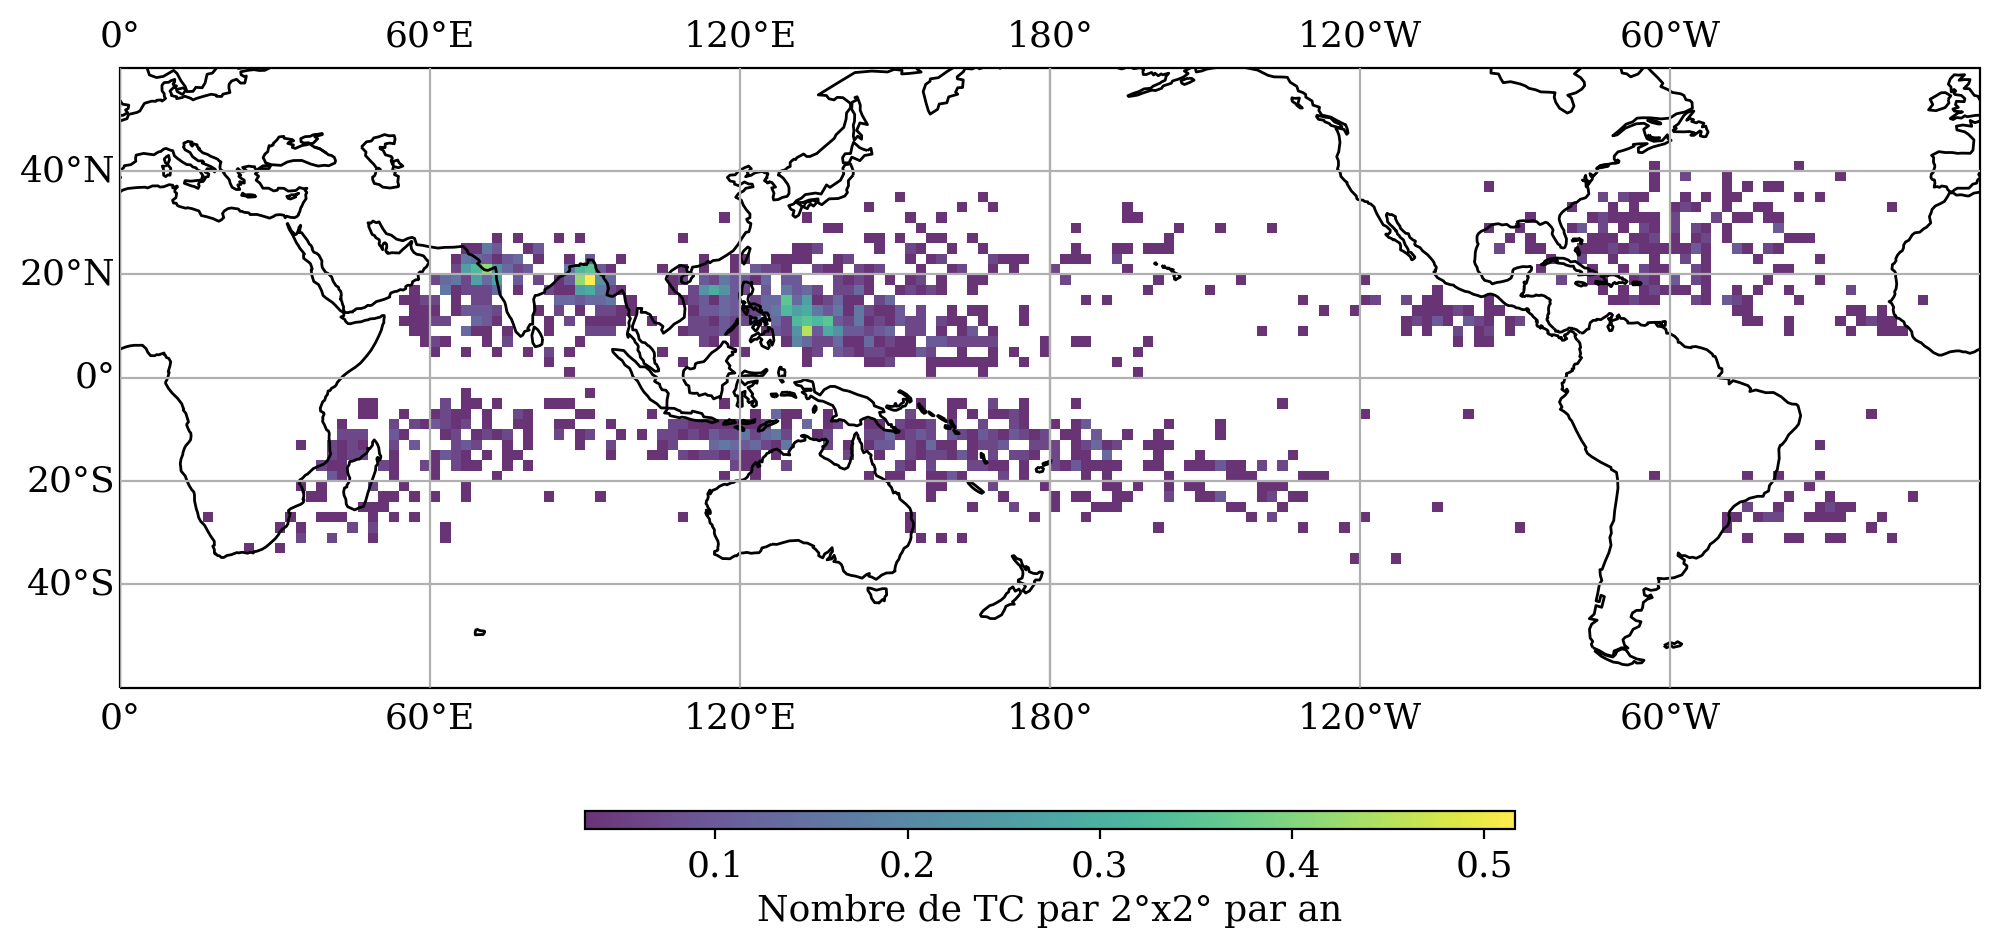
\includegraphics[width=\textwidth]{track_density_PRE625REFT359x.png}
    \caption{Densité annuelle moyenne de cyclogénèses dans la simulation ARPEGE forcée par HadISST1 entre 1980 et 2010, calculée sur une grille régulière de
    \ang{2}$\times$\ang{2}.}
    \label{fig:track_density_PRE625REFT359x}
\end{figure}
%
\begin{figure}[tp]
    \centering
    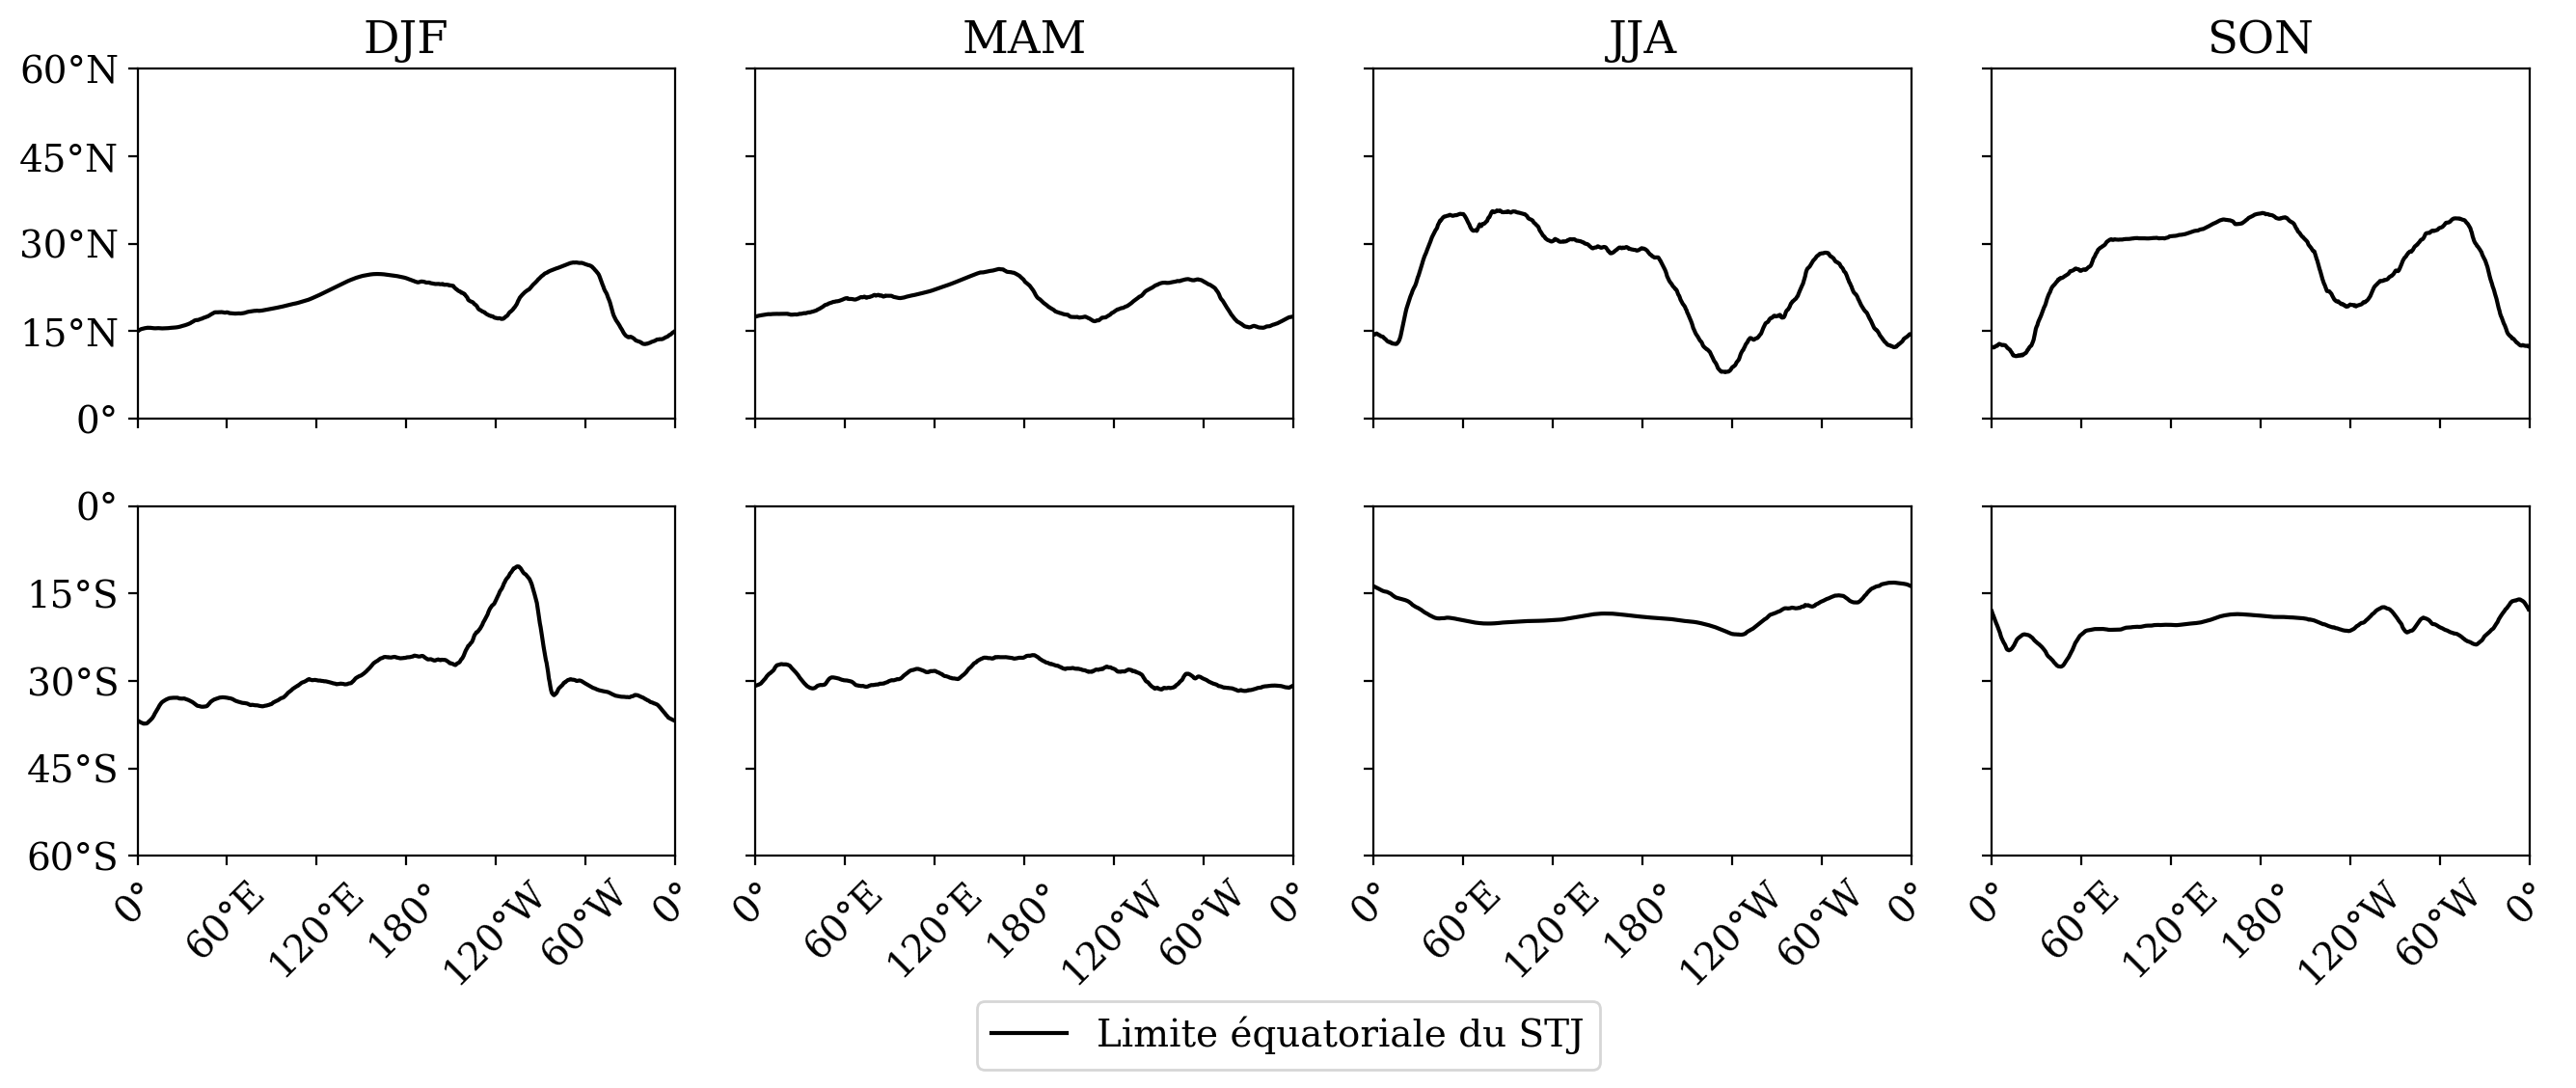
\includegraphics[width=\textwidth]{STJ_season_PRE625REFT359x.png}
    \caption{Moyennes saisonnières de la latitude de la limite équatoriale du jet subtropical dans la simulation ARPEGE-Climat forcée par HadISST1. Chacune des
    quatre colonnes correspond à une saison. La première ligne présente le diagnostique pour l'hémisphère nord, tandis que la seconde ligne le présente pour
    l'hémisphère sud.}
    \label{fig:STJ_PRE625REFT359x}
\end{figure}

\section{Tendances}

%--------------------------------------
\section{Synthèse}

\end{document}
